%\documentclass{beamer}
\documentclass[11ppt]{beamer}



% ***********************************************************
% ******************* PHYSICS HEADER ************************
% ***********************************************************
% Version 2

\usepackage{amsmath} % AMS Math Package
\usepackage{amsthm} % Theorem Formatting
\usepackage{amssymb}	% Math symbols such as \mathbb
\usepackage{graphicx} % Allows for eps images
\usepackage{multicol} % Allows for multiple columns
\usepackage[dvips,showframe,letterpaper,margin=1.0in,left=1.5in]{geometry}
% tim included
\usepackage[pdftex,bookmarks=true]{hyperref}

\usepackage{cancel}
\usepackage{siunitx}
 % Sets margins and page size
\pagestyle{plain} % Removes page numbers
\makeatletter % Need for anything that contains an @ command 
\renewcommand{\maketitle} % Redefine maketitle to conserve space
{ \begingroup \vskip 10pt \begin{center} \large {\bf \@title}
	\vskip 10pt \large \@author \hskip 20pt \@date \end{center}
  \vskip 10pt \endgroup \setcounter{footnote}{0} }
\makeatother % End of region containing @ commands
\renewcommand{\labelenumi}{(\alph{enumi})} % Use letters for enumerate
% \DeclareMathOperator{\Sample}{Sample}
\let\vaccent=\v % rename builtin command \v{} to \vaccent{}
\renewcommand{\v}[1]{\ensuremath{\mathbf{#1}}} % for vectors
\newcommand{\gv}[1]{\ensuremath{\mbox{\boldmath$ #1 $}}} 
% for vectors of Greek letters
\newcommand{\uv}[1]{\ensuremath{\mathbf{\hat{#1}}}} % for unit vector
\newcommand{\abs}[1]{\left| #1 \right|} % for absolute value
\newcommand{\avg}[1]{\left< #1 \right>} % for average
\let\underdot=\d % rename builtin command \d{} to \underdot{}
\renewcommand{\d}[2]{\frac{d #1}{d #2}} % for derivatives
\newcommand{\dd}[2]{\frac{d^2 #1}{d #2^2}} % for double derivatives
\newcommand{\pd}[2]{\frac{\partial #1}{\partial #2}} 
% for partial derivatives
\newcommand{\pdd}[2]{\frac{\partial^2 #1}{\partial #2^2}} 
% for double partial derivatives
\newcommand{\pdc}[3]{\left( \frac{\partial #1}{\partial #2}
 \right)_{#3}} % for thermodynamic partial derivatives
\newcommand{\ket}[1]{\left| #1 \right>} % for Dirac bras
\newcommand{\bra}[1]{\left< #1 \right|} % for Dirac kets
\newcommand{\braket}[2]{\left< #1 \vphantom{#2} \right|
 \left. #2 \vphantom{#1} \right>} % for Dirac brackets
\newcommand{\matrixel}[3]{\left< #1 \vphantom{#2#3} \right|
 #2 \left| #3 \vphantom{#1#2} \right>} % for Dirac matrix elements
\newcommand{\grad}[1]{\gv{\nabla} #1} % for gradient
\let\divsymb=\div % rename builtin command \div to \divsymb
\renewcommand{\div}[1]{\gv{\nabla} \cdot #1} % for divergence
\newcommand{\curl}[1]{\gv{\nabla} \times #1} % for curl
\let\baraccent=\= % rename builtin command \= to \baraccent
\renewcommand{\=}[1]{\stackrel{#1}{=}} % for putting numbers above =
\newtheorem{prop}{Proposition}
\newtheorem{thm}{Theorem}[section]
\newtheorem{lem}[thm]{Lemma}
\theoremstyle{definition}
\newtheorem{dfn}{Definition}
\theoremstyle{remark}
\newtheorem*{rmk}{Remark}

% ***********************************************************
% ********************** END HEADER *************************
% *********************************************************** 
\usetheme{Copenhagen}
\newcommand{\sr}{u}
\newcommand{\srb}{\bar{u}}
\newcommand{\wx}{\phi}
\newcommand{\wxd}{\phi^\dagger}

\newcommand{\W}{w}

\newcommand{\smalldot}{\cdot}


\newcommand{\beqa}{\begin{eqnarray*} }
\newcommand{\eeqa}{\end{eqnarray*} }
\newcommand{\beq}{\begin{equation*} }
\newcommand{\eeq}{\end{equation*} }
\newcommand{\beqB}{\begin{equation*}}
\newcommand{\eeqB}{\end{equation*}}

 \newcommand{\epin}[1]{ \epsilon_{#1}(p) }
 \newcommand{\epout}[1]{ \epsilon^*_{#1}(p') }
\newcommand{\omin}[1]{ \W_{#1}(p) }
 \newcommand{\omout}[1]{ \W^*_{#1}(p') }



\newcommand{\Sitem}[1]{ \begin{itemize} \item #1 \end{itemize} }

\title{Universal Binding and Recoil Corrections to Bound State g-Factors}

%TODO add eides, affiliation
\author{Tim Martin}
\date{May 26th, 2011}
\institute{University of Kentucky}

\begin{document}

\begin{frame}
	\titlepage
\end{frame}







%Slide 1
\begin{frame}{Background}



\begin{itemize}
% Even in free case, g-factors often not determined by electromagnetic origin

% Clarify: Loosely bound two particle systems


\item Corrections to g-factor of bound particles are well established for spin-1/2
\pause
\item Measurements in hydrogen-like carbon $^{12}C^{5+}$ or oxygen $^{16} O^{7+}$ need a precise theoretical bound $g$-factor, and involve systems with nuclear spin 0
\pause
\item We find leading order recoil and binding corrections for particles of arbitrary spin

\end{itemize}
\end{frame}

\begin{frame}
\frametitle{Definition of $g$}
	\begin{itemize}
	  \item	Gyromagnetic ratio: ratio of \textbf{magnetic dipole moment} to \textbf{angular momentum}
	  \item Here, concerned only with the gyromagnetic ratio associated with spin
	  \item Then $g$-factor related to magnetic moment by
	  	\beq	\gv{\mu} = g \frac{e}{2m} \v{S} \eeq
	  \item	Energy difference between spin-flipped states
	  	\beq
			\Delta E =  g \frac{e}{m} \v{S} \cdot \v{B}.
		\eeq
	\end{itemize}
\end{frame}

\begin{frame}
\frametitle{Free $g$-factor}
	\begin{itemize}
	  \item	Free $g$-factor well known for electron
	  \item Leading order $g=2$, modified by radiative corrections
	  
	  \vskip 1em
	\mbox{
	\begin{minipage}{.5in}
	  \begin{center} 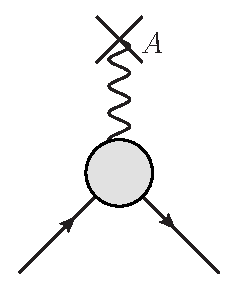
\includegraphics[scale=0.3]{../eps/QED-static-field-blob} \end{center} 
	\end{minipage}
	=
	\begin{minipage}{.5in}
	   \begin{center}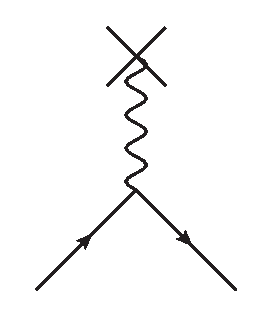
\includegraphics[scale=0.3]{../eps/QEDfund}\end{center} 
	\end{minipage}
	+
	\begin{minipage}{.5in}
	   \begin{center} 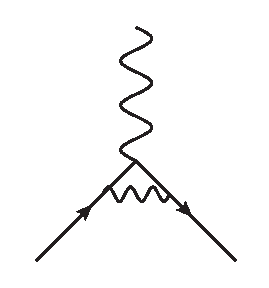
\includegraphics[scale=0.3]{../eps/QEDloop1} \end{center} 
	\end{minipage}
	+
	\begin{minipage}{.5in}
	   \begin{center} 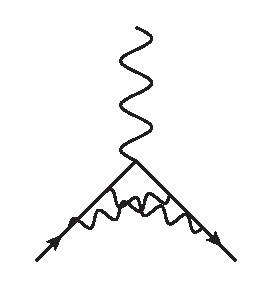
\includegraphics[scale=0.3]{../eps/QEDloop2} \end{center} 
	\end{minipage}
	+ \hspace{2em} $\cdots$
	 }
	\vspace{1em} 
	\item Theoretical value agrees well with the measured value, (Hanneke, Fogwell, Gabrielse, 2008):
		\beq
			g_e = \num{2.002 319 304 3622(15)},    \hspace{2em} \delta = 7.4 \times 10^{-13}.
		\eeq
	\end{itemize}


\end{frame}

\begin{frame}
\frametitle{Bound $g$-factor}
For a particle in a bound state, there are corrections besides radiative.
\begin{itemize}
 \item 	Recoil corrections that occur when separating the internal degrees of freedom from the external motion of the whole system.  (Order $m/M$)
  \item 	Relativistic or binding corrections.  (Because the velocity of a hydrogenic bound system is $v \sim Z\alpha$, corrections of this nature will be an expansion over $(Z\alpha)^2$)
  \item		Additional effect such as due to the finite size of the nucleus --- not considered here.
\end{itemize}
\end{frame}

\begin{frame}
\frametitle{Bound $g$-factor}
\begin{itemize}
  \item Binding corrections for the electron with $g=2$ first calculated by Breit (1928)
  \item Calculating $\avg{ e\gamma \cdot A}$ gives
  		\beq 
			g_b =  \frac{2}{3}\left( 1 + 2 \sqrt{1 - (Z\alpha)^2}\right)  = 2 \left( 1 - \frac{(Z\alpha)^2}{3} - \frac{(Z\alpha)^4}{12}  + \cdots \right )
		\eeq	
  \item	For systems with nuclear spin one-half, the situation is well understood.  For instance up to order $\alpha (Z\alpha)^2$:
		\footnotesize \beq \begin{split}
	g_b = &g_e \Big \{ 1 - \frac{1}{3} (Z\alpha)^2 \left[ 1 - \frac{3}{2} \frac{m}{M} + \frac{3}{2}(1+Z) \frac{m^2}{M^2} \right ]
		\\& + \frac{1}{4\pi} \alpha (Z\alpha)^2 \left[ 1 - \frac{5}{3} \frac{m}{M} + \frac{6+Z}{3} \frac{m^2}{M^2} \right ] \Big \}.
		\end{split}
\eeq \normalsize
	\item In general, corrections as a series in $\alpha^n (Z\alpha)^k$ and $(m/M)$.
	\item But, a result for arbitrary spin is needed 
\end{itemize}
  
\end{frame}


\begin{frame}
\frametitle{Experiment}
 


\begin{itemize}
  \item	Hydrogen like ion is placed in a weak magnetic field $B$
  \item Spin flip frequency $\omega_L$, corresponding to transitions between Zeeman levels, is measured
   	\beq
		\omega_L = g_b \frac{e}{2m_e} B.
	\eeq
  \item The cyclotron frequency $\omega_C$ is
	\beq
		\omega_C = (Z-1) \frac{eB}{M}.
	\eeq
	\item Ratio can determine $g_b$
	\beq
		\frac{\omega_L}{\omega_C} = \frac{f_L}{f_C} = 
		g_b \frac{e}{2(Z-1)} \frac{M}{m_e}.
	\eeq	
	\item Or, determine electron mass
		\beq
			m_e = \frac{g_b}{2(Z-1)} \frac{\omega_C}{\omega_L} M
		\eeq
\end{itemize}
\end{frame}

\begin{frame}
\frametitle{Measurements}
	\begin{itemize}
	  \item Most sensitive experiments in carbon $^{12}C^{5+}$ or oxygen $^{16} O^{7+}$ (Haffner, Werth, Verdu, 2003)
	  \item Carbon
	  	\small \beq
			 \frac{f_L}{f_C} = \num{4376.2104989(23)},	\hspace{3em} 	\delta= 5.2 \times 10^{-10}.
		\eeq \normalsize
	  \item Oxygen
		\small \beq
				 \frac{f_L}{f_C} = \num{4 164.376 1837 (32)}, \hspace{3em} \delta= 7.6 \times 10^{-10}.
		\eeq \normalsize
		\item Precise enough to be best source of electron mass ratio
		\begin{itemize}
		  \item Already factor of 5 improvement over previous result
		  \item Experiments with smaller errors will further improve measurement
		\end{itemize}
		\item But, requires theoretical value of $g_b$ with enough precision
	\end{itemize}
\end{frame}



\begin{frame}
\frametitle{Statement of problem}
\begin{itemize}
  \item Consider loosely bound hydrogen-like systems, in a weak, constant magnetic field
  \item Calculate leading binding and recoil corrections to $g_b$
  \item Binding corrections will be of order $(Z\alpha)^2$ relative to zero-order value
\end{itemize}
\end{frame}





\begin{frame}
\frametitle{Approach}

\begin{itemize}

\item	\emph{Goal}: calculate leading binding and recoil corrections to the bound gyromagnetic ratio

\item 	Possible if an effective nonrelativistic Lagrangian was known to order $1/m^3$

\item 	\emph{Strategy}: 
\begin{itemize}
  	\item 	Write down the most general form of such a Lagrangian, and fix the coefficients by comparing to relativistic theory
	\item 	Then use this to calculate the interaction potential
	\item 	From the interaction potential can be found $g_b$.
\end{itemize}
\end{itemize}

\end{frame}

\begin{frame}
\frametitle{Approach}
Work through this approach in several contexts:
\begin{itemize}
\item<1->	First, consider well known case --- a spin one-half particle like the electron.

\item<2-> 	Next move to a spin one particle, such as the W boson.

\item<3-> 	Finally derive an effective Lagrangian valid for arbitrary spin, and compare the result to the specific cases.

\end{itemize}

\vspace{2em}
% \begin{columns}
% \column{1in}<1->
% $s=\frac{1}{2}$
% \column{1in}<2->
% $s=1$
% \column{1in}<3->
% $s= ?$
% \end{columns}

\end{frame}

\begin{frame}
\frametitle{How to construct an effective Lagrangian}
\begin{itemize}
\item 	Finite number of fields and operators to construct terms in the Lagrangian
\item 	Combinations of these terms are restricted by symmetries and other constraints of the theory (Hermiticity, gauge invariance, etc.)
\item 	Still an infinite number of combinations
\item 	But, at a given level of precision, only a finite number of relevant terms
\item 	Write down a Lagrangian with all such terms: 
\item	Result: a Lagrangian with several coefficients, capturing the details of the high energy/small scale physics
\item 	Fix these coefficients (to some level of precision) by demanding consistency with the higher energy theory.
\end{itemize}
\end{frame}

\begin{frame}
\frametitle{Constructing the effective NRQED Lagrangian for spin one-half}
\begin{itemize}
  
\item	Constraints: Invariance under Galilean transforms as well as parity and time reversal, Hermiticity, and gauge invariance
\item Gauge invariance will be fulfilled automatically if we use only gauge invariant building blocks with which to construct the Lagrangian
\item In addition to the fermion field $\psi$, several other building blocks:
\begin{center}
	$\v{S}$, $\v{E}$, $\v{B}$, and $\v{D} = \v{\grad} - ie\v{A}$
\end{center}
\item  For our purposes, only the interaction of a single charged particle with an electromagnetic field is needed.  So all terms in the Lagrangian will involve two fermion fields, with various powers of the other building blocks.
\end{itemize}
\end{frame}

\begin{frame}
\frametitle{Restrictions on relevance of terms}
\begin{itemize}
\item To calculate the leading ($v^2 \sim (Z\alpha)^2$) binding corrections to $g_b$, only leading order corrections in the Lagrangian need be considered
\item The original nonrelativistic Lagrangian is
\end{itemize}
 
%FIXME correct lagrangian
\begin{equation}
	\mathcal{L} = D_0 + \frac{ \v{D}^2}{2m}  - g \frac{e}{2m} \v{S} \cdot \v{B}
\end{equation}
\begin{itemize}
\item For a hydrogen like system, it contains terms of $\mathcal{O}(mv^2)$ and $\mathcal{O}(B/m)$.  
\item So the corrections needed will be $\mathcal{O}(mv^4)$ and $\mathcal{O}(v^2 B/m)$. 
\item Terms quadratic in the magnetic field may be neglected
\end{itemize}
\end{frame}




%\begin{frame}
%\frametitle{NRQED Lagrangian}
%Want to write down all terms in NRQED Lagrangian that contribute to final result --- terms of $O(1/m^3)$

%Building blocks of the Lagrangian are S, B, E, $D_i$, and $D_0$ 

%Different arrangements of these terms give the various terms in the lagrangian.  What are the orders of these terms?

%\beq
%	S \sim 1, E \sim m^2v^3, B \text{is its own scale, but small}, D_i \sim mv, D_0 \sim mv^2
%\eeq
% 
% In spin one-half, there are no terms quadratic in spin, $S_i S_j$ reduces to $\delta_{ij} + i\epsilon_{ijk}S_k$.  
% 
% Consider combinations which are Hermitian, invariant under parity rotation and time reversal, and have mass dimension 4..
% 
% Allowed term: $ c_D \psi^\dagger\frac{ \v{D} \cdot \v{E} - \v{E} \cdot \v{D}}{8m^2} \psi$.
% 
% Terms can always be constructed to have the right properties under Hermiticity/time reversal, but parity can forbid some combinations: no way to make a term like $ \v{S} \cdot \v{D}$, for instance.
% \end{frame}

\begin{frame}
\frametitle{ NRQED Lagrangian }
All the allowed terms are

\only<1>{
\footnotesize{

\beq 
\begin{split}
\mathcal{L}_{NRQED} = & \psi^\dagger \Bigg\{
		iD_0 +  \frac{\v{D}^2}{2m}  + 	\frac{\v{D}^4}{8m^2}
		 + c_F \frac{e}{m} \v{S} \cdot \v{B}
		+ c_D \frac{e (\v{D} \cdot \v{E} - \v{E} \cdot \v{D})}{8m^2} 
\\&	 + c_S \frac{ i e \v{S} \cdot(\v{D} \times \v{E} - \v{E} \times \v{D}) }{8m^2}
		+ c_{W1} \frac{ e \v{D}^2 (\v{S} \cdot \v{B}) + (\v{S} \cdot \v{B}) \v{D}^2 }{8m^3}
\\	&		- c_{W2} \frac{e D_i (\v{S} \cdot \v{B}) D_i}{4m^3}
		+c_{p'p} \frac{ e [ (\v{S}\cdot \v{D})(\v{B} \cdot \v{D}) + (\v{B} \cdot \v{D})(\v{S}\cdot \v{D})]}{8m^3}
		\Bigg \} \psi
\end{split}
\eeq }}
\only<2>{
\footnotesize{

\beq 
\begin{split}
\mathcal{L}_{NRQED} = & \psi^\dagger \Bigg\{
		iD_0 +  \frac{\v{D}^2}{2m}  + 	\frac{\v{D}^4}{8m^2}
		 + c_F \frac{e}{m} \v{S} \cdot \v{B}
		+ c_D \frac{e (\v{D} \cdot \v{E} - \v{E} \cdot \v{D})}{8m^2} 
\\&	 + c_S \frac{ i e \v{S} \cdot(\v{D} \times \v{E} - \v{E} \times \v{D}) }{8m^2}
		+ (c_{W1} - c_{W2}) c_{W2} \frac{e D_i (\v{S} \cdot \v{B}) D_i}{4m^3}
\\	&		+c_{p'p} \frac{ e [ (\v{S}\cdot \v{D})(\v{B} \cdot \v{D}) + (\v{B} \cdot \v{D})(\v{S}\cdot \v{D})]}{8m^3}
		\Bigg \} \psi
\end{split}
\eeq}

(Considering only constant magnetic field)
}





\end{frame}

\begin{frame}
\frametitle{Scattering comparison}
\begin{itemize}
  \item Fix coefficients by comparison of physical processes
  \item Only need coefficients in front of one-photon terms
  \item (Terms like $\v{E} \times \v{A}$ contribute, but are part of gauge invariant $\v{E} \times \v{D}$ )
  \item Elastic scattering off external field fixes all desired terms
  \item Also use stronger constraint that magnetic field is constant
\end{itemize}

\vspace{1em}
 \mbox{


$\underbrace{ \begin{minipage}{1in}
   \center{    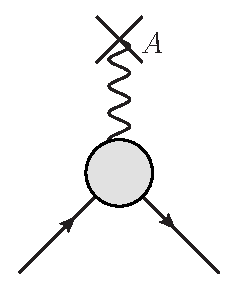
\includegraphics[scale=0.5]{../eps/QED-static-field-blob}   } 
\end{minipage} }_{\text{QED}} 
	=	\hspace{1em} 	 
 \underbrace{ \begin{minipage}{1in}
  \center{   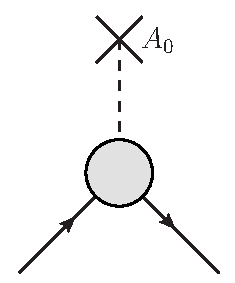
\includegraphics[scale=0.5]{../eps/NRQED-static-coulomb-field}    }
\end{minipage}
 \hspace{1em}   +  \hspace{1em}  
\begin{minipage}{1in}
  \center{   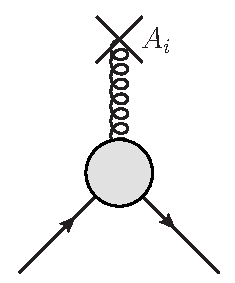
\includegraphics[scale=0.5]{../eps/NRQED-static-vector-field}   }  
\end{minipage}  }_{\text{NRQED}} $
} 
\vspace{1em}


\end{frame}

\begin{frame}
\frametitle{Scattering in QED --- form of vertex}
\begin{overprint}
\begin{itemize}
	\item QED one-photon scattering
	\item Form of vertex captured by just two form factors
	\item  $ iM =-ie  \bar{u} \Gamma^\mu A_\mu u$, $\Gamma^\mu$ defined as:
\end{itemize}
\end{overprint}
	\only<1>{\beq
		\Gamma^\mu = F_1(q^2) \gamma^\mu + F_2(q^2) \frac{ i \sigma^{\mu\nu}q_\nu}{2m} 
	\eeq}
	\only<2>{
	\beq
		\Gamma^\mu = F_1(q^2) \frac{p^\mu  + p'^\mu }{2m}  +  i [F_1(q^2) + F_2(q^2) ] \frac{\sigma^{\mu\nu}q_\nu}{2m}  .
	\eeq}	
\end{frame}

\begin{frame}
\frametitle{Scattering in QED --- relationship between $u$ and $\phi$}
\begin{itemize}
	\item Relation between $u$ and $\phi$?
	\item Demand that current densities match at 0 momentum transfer ($q=0$)
\end{itemize}
	\beq
		e  \frac{p^0}{m} \bar{u} u = e \phi^\dagger \phi, \hspace{3em} \text{where }		u = \begin{pmatrix} \eta \\ \chi \end{pmatrix} = \begin{pmatrix} \eta \\ \frac{ \gv{\sigma} \cdot \v{p} }{2m} \eta \end{pmatrix}
	\eeq
 Discarding terms of $\mathcal{O}(\v{p}^4 / m^3)$
%	\beq
%		 e  \left( 1 + \frac{\v{p}^2}{2m^2} \right ) \eta^\dagger \left( 1 - \frac{ \gv{\sigma} \cdot \v{p} }{2m}   \right )^2 \eta \approx e \phi^\dagger \phi
%	\eeq
	 
	\beq
		 \eta \approx \left( 1 - \frac{\v{p}^2}{8m^2} \right ) \phi
	\eeq
	

\end{frame}

\begin{frame}
\frametitle{Scattering in QED --- amplitudes in terms of $\phi$}

\begin{itemize}
  \item $\bar{u} \Gamma^\mu u$ in terms of $\phi$
\end{itemize}
\footnotesize
\beqa 
	(p + p')^\mu \bar{u} u  &=& (p + p')^\mu \phi^\dagger \left( 
		1 -  \frac{ \v{p}^2  +2 \v{p} \cdot \v{p'} +  \v{p'}}{8m^2} - \frac{i\gv{\sigma} \cdot \v{q} \times \v{p} }{4m^2} 
		\right ) \phi \\
	\srb  \frac{i}{2m} q_j \sigma^{ij} \sr 
		&=& \frac{i \epsilon_{ijk} q_j}{2m} \wxd \left (
			\sigma_k - \frac{ \gv{\sigma} \cdot \v{p} p_k  }{2m^2} 
		\right ) \wx	\\
 \srb  \frac{i}{2m} q_j \sigma^{0j} \sr
	&=&  -  \wxd \left (
			\frac{  \v{q}^2  }{4m^2} 
			- \frac{  i\gv{\sigma} \cdot \v{q} \times \v{p}   }{2m^2} 
	\right ) \wx
\eeqa
\normalsize

\end{frame}
\begin{frame}
\frametitle{Scattering in QED --- amplitudes in terms of $\phi$}
Amplitudes:
\footnotesize
\beq
		 eA_0 \srb  \Gamma^0 \sr = \wxd \left(  
			F_1  eA_0
			+ [F_1 + 2 F_2] \left [ 
				\frac{e \gv{\sigma} \cdot \v{E} \times \v{p} }{4m^2}  - \frac{e  \grad \cdot \v{E} }{8m^2}
			\right ]
		\right ) \wx,
\eeq

\beq \begin{split}
	e A_i \srb \Gamma^i \sr =  \wxd \Bigg \{
		- F_1 \frac{ e\v{A} \cdot (\v{p} + \v{p'} ) }{2m} \left( 1 - \frac{\v{p}^2}{2m^2} \right )
		- [F_1 + F_2] \frac{ e \gv{\sigma} \cdot \v{B} }{2m} 
	\\	+ F_1 \frac{ e \gv{\sigma} \cdot \v{B} \v{p}^2 }{4m^3} 
		+ F_2 \frac{ (\gv{\sigma} \cdot \v{p}) (\v{B} \cdot \v{p}) }{4m^2}
	\Bigg \} \wx.
\end{split}
\eeq
\normalsize
\end{frame}

\begin{frame}
\frametitle{Scattering in NRQED}
	\begin{itemize}
	  \item One photon scattering read directly from Lagrangian
	  \item For instance, $\v{D}^2 \to  e (\v{p} + \v{p}') \cdot \v{A} $ 
	\end{itemize}
	
	\begin{block}{Nonrelativistic amplitude}
	\footnotesize \beq 
\begin{split} 
	iM =&
		ie\phi^\dagger \Bigg(  -A_0 +  \frac{ \v{A} \cdot (\v{p} + \v{p}') }{2m} - \frac{  \v{A} \cdot (\v{p} + \v{p'}) \v{p}^2   }{4m^3} 
		+ c_F  \frac{\v{S} \cdot \v{B}} {2m}   	
		+ c_D \frac{ ( \partial_i E_i ) }{8m^2}	
		\\&	+ c^{1}_S \frac{  \v{E} \times \v{p} }{4m^2}
		- (c_{W_1} -c_{W_2}) \frac{   (\v{S} \cdot \v{B} ) \v{p}^2  }{4m^3}	
		-  c_{p'p} \frac{   (\v{S} \cdot \v{p}) (\v{B} \cdot \v{p})  }{4m^3} \Bigg )\phi .
\end{split}
\eeq \normalsize
	\end{block}
\end{frame}

\begin{frame}
\frametitle{Coefficients}

	Comparing the two, coefficients are:
	\begin{block}{Coefficients for spin one-half}
\begin{columns}[l]
\column{.5 in}
\beqa
	c_F &=& g \\
	c_D &=&	(g-1) 	\\
\eeqa
\column{1 in}
\beqa
	c_S &=& 2(g-1)	\\
	c_{W_1}- c_{W_2} &=& 2	\\
	c_{p'p}	&=&  g-2	
\eeqa
\end{columns}
	\end{block}

\end{frame}

\begin{frame}
\frametitle{Spin one}
	\begin{itemize}
	  \item Same type of calculation can be done for a spin one particle
	  \item Standard model contains $W^+$, $W^-$
	  \item Known relativistic Lagrangian, so no obstacles in calculating scattering
	  \item NRQED Lagrangian for spin one will contain new terms
	\end{itemize}

\end{frame}


\begin{frame}
\frametitle{NRQED Lagrangian for spin one}
\begin{itemize}
  \item Same building blocks as before
  \item All terms from spin one-half exist here, too
  \item New terms arise because quadratic spin terms are allowed
  \item Quadrupole moment $Q_{ij} = S_i S_j + S_j S_i - \frac{2}{3} \delta_{ij} \v{S}^2$
\end{itemize}
One new term
	\beq
		c_Q \frac{ Q_{ij} (D_i E_j - E_j D_i) }{8m^3}
	\eeq
\end{frame}
\begin{frame}
\frametitle{NRQED Lagrangian}
General form for spin one NRQED Lagrangian is:
\footnotesize 
\beq
\begin{split}
	\mathcal{L}_{NRQED} = \psi^\dagger \Bigg \{ & i(\partial_0 + ieA_0) + \frac{\v{D}^2}{2m} + \frac{\v{D}^4}{8m^3} 
		+ c_F e \frac{\v{S} \smalldot \v{B}} {2m}   	
		+ c_D \frac{ e(\v{D} \smalldot \v{E} - \v{E} \smalldot \v{D} ) }{8m^2}	
	\\&	+ c_Q \frac{e Q_{ij} (D_i E_j - E_i D_j) }{8m^2}	
		+ c_S \frac{ ie \v{S} \smalldot ( \v{D} \times \v{E} - \v{E} \times \v{D} )}{8m^2}
	\\&	+ (c_{W_1}- c_{W_2}) \frac{ e  (\v{S} \smalldot \v{B} ) \v{D}^2 }{4m^3}
		+ c_{p' p} \frac{ e [ (\v{S} \smalldot \v{D}) (\v{B} \smalldot \v{D}) + (\v{B} \smalldot \v{D})(\v{S} \smalldot \v{D}) }{8m^3} \Bigg \} \psi
\end{split}
\eeq

\normalsize
\end{frame}


\begin{frame}[t]
\frametitle{Relativistic scattering  --- diagrams}
 
\begin{block}{Relativistic Lagrangian}

\footnotesize
\beq 
\mathcal{L} 
	=	-\frac{1}{2} (D^\mu W^\nu - D^\nu W^\mu)^\dagger (D_\mu W_\nu - D_\nu W_\mu)
		+ m^2 W^{\mu \dagger} W_\mu - i [g-1] e  W^{\mu \dagger} W^\nu F_{\mu\nu}
\eeq
\normalsize


\end{block}

\only<1>
{From the above Lagrangian, derive Feynman rules and current density} 

\only<2>{
Diagrams are
\vspace{1em}

\footnotesize 
\mbox{
\begin{minipage}{1in}
   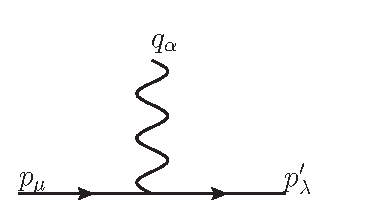
\includegraphics[scale=0.5]{../eps/one-photon-fundamental} 
\end{minipage}
$=$
\begin{minipage}{2in}
\beq \begin{split}
   -ie\Big [ g^{\mu\lambda}(p + p')^\alpha - g^{\lambda \alpha} (p' + [g-1]q)^\mu 
      \\- g^{\alpha \mu} (p - [g-1]q)^\lambda \Big ]
\end{split}\eeq 
\end{minipage}
}

\vspace{3em}

\mbox{
\begin{minipage}{1in}
   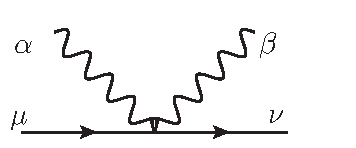
\includegraphics[scale=0.5]{../eps/two-photon-fundamental} 
\end{minipage}
$	=	 -i e^2 ( 2 g^{\mu\nu} g^{\alpha \beta} - g^{\mu \beta} g^{\nu \alpha} - g^{\nu\beta}g^{\mu\alpha}) $
}
\normalsize
}

\only<3>{
External charged particle legs
\vspace{3em}

\begin{columns}[c]
\column{1.5in}
\mbox{
\begin{minipage}{1in}
   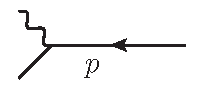
\includegraphics[scale=0.7]{../eps/ParticleInitial} 
\end{minipage}
$= \W_\mu(p)$
}

\mbox{
\begin{minipage}{1in}
   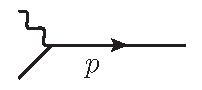
\includegraphics[scale=0.7]{../eps/ParticleFinal} 
\end{minipage}
$= \W^*_\mu(p)$
}


\column{1.5in}
\beq 
	p \cdot \W(p) = 0
\eeq
\end{columns}

}


\end{frame}


\begin{frame}
\frametitle{Amplitudes in terms of $\phi$}
Again, $j_0(q=0)$ must match.
\beq
	 \phi^\dagger \phi = 2 p_0 \gv{\W}^\dagger \cdot \gv{\W} - 2 \frac{ ( \gv{\W}^\dagger \cdot \v{p})( \v{p} \cdot \gv{\W} )}{p_0}
\eeq 
Mixing between components can be written as the action of spin operators
\beq \begin{split}
	\gv{\W} =
		 \frac{1}{\sqrt{2m}} \left (1 + \frac{ \v{p}^2}{4m^2} - \frac{(\v{S} \cdot \v{p})^2 }{2m^2} \right ) \phi
\end{split} \eeq




\end{frame}

\begin{frame}
\frametitle{QED amplitude}
\begin{itemize} \item Amplitude from single vertex \end{itemize}
\beq
	iM = ie \omin{\mu} \omout{\nu} \left[ g^{\mu\nu} (p + p')\cdot A  +g ( q^\nu A^\mu - q^\mu A^\nu ) \right] 	
\eeq
\begin{itemize} 
   \item Split into two parts
   \item First has no $g$ dependence 
   \beq
	M_q = ie \omin{\mu} \omout{\nu} g^{\mu\nu} (p + p')\cdot A 
\eeq
   \item Second proportional to $g$
\beq
	M_g = ie g  \omin{\mu} \omout{\nu}  ( q^\nu A^\mu - q^\mu A^\nu ) 	
\eeq

\end{itemize}


\end{frame}

\begin{frame}
\frametitle{QED amplitude}
\begin{itemize}
\item Work out the nonrelativistic approximation as before
\item Result:
\end{itemize}
\begin{block}{QED amplitude}
\footnotesize
\beq 
\begin{split}
iM_{REL} =& -ie \phi^\dagger \Big (
		 A_0  - \frac{\v{p}\cdot \v{A} }{m} + \frac{\v{p}\cdot \v{A} \v{p}^2}{2m^3}
		- \frac{g-1}{2m^3}\{ \grad \cdot \v{E} -  \v{S} \cdot \v{p} \times \v{E} - S_i S_j \grad_i E_j \}
		\\& - g\frac{1}{2m} \v{S} \cdot \v{B}
		+ \v{S} \cdot \v{B} \frac{\v{p}^2}{2m^3}
		+ \frac{g-2}{4m^3}(\v{S} \cdot \v{p} )( \v{B} \cdot \v{p})
	\Big ) \phi
\end{split}
\eeq
\normalsize
\end{block}
\end{frame}


\begin{frame}
\frametitle{NRQED Amplitude}
\Sitem{Again, read off one photon scattering from the NRQED Lagrangian}
\begin{block}{NRQED Amplitude}
\footnotesize
\beqa
	iM &=&
		ie\phi^\dagger \Bigg(  -A_0 +  \frac{ \v{A} \cdot \v{p} }{m} - \frac{  (\v{A} \cdot \v{p}) \v{p}^2   }{2m^3} 
		+ c_F  \frac{\v{S} \smalldot \v{B}} {2m}   	
		+ c_D \frac{ ( \partial_i E_i ) }{8m^2}	
		+ c_Q \frac{ Q_{ij} ( \partial_i E_j ) }{8m^2}	
	\\&&	+ c_S \frac{  \v{E} \times \v{p} }{4m^2}
		- (c_{W_1} -c_{W_2}) \frac{   (\v{S} \smalldot \v{B} ) \v{p}^2  }{4m^3}	
		-  c_{p'p} \frac{   (\v{S} \smalldot \v{p}) (\v{B} \smalldot \v{p})  }{4m^3} \Bigg )\phi
\eeqa
\normalsize
\end{block}
\end{frame}

\begin{frame}
\frametitle{Coefficients}

\Sitem{Comparing the two amplitudes, the coefficients are fixed}

\begin{block}{Spin one coefficients}
\begin{columns}[l]
\column{.5 in}
\beqa
	c_F &=& g \\
	c_D &=&	\frac{4(g-1)}{3} 	\\
	c_Q &=&	-4 (g-1)	
\eeqa
\column{1 in}
\beqa
	c_S &=& 2(g-1)	\\
	c_{W_1}- c_{W_2} &=& 2	\\
	c_{p'p}	&=&  g-2	
\eeqa
\end{columns}
\end{block}
\pause
\Sitem{	For contrast, the spin half coefficients were}

\begin{block}{Spin half coefficients}
\begin{columns}[l]
\column{.5 in}
\beqa
	c_F &=& g \\
	c_D &=&	(g-1) 	\\
\eeqa
\column{1 in}
\beqa
	c_S &=& 2(g-1)	\\
	c_{W_1}- c_{W_2} &=& 2	\\
	c_{p'p}	&=&  g-2	
\eeqa
\end{columns}
	\end{block}
\end{frame}


\begin{frame}
\frametitle{Arbitrary spin}
Now we move on to a formalism for particles of arbitrary spin
\begin{itemize}
  \item First develop NRQED Lagrangian
  \item Then an effective relativistic theory
\end{itemize}
\end{frame}

\begin{frame}{NRQED Lagrangian}

\begin{itemize}
  \item For the case of general spin, more complicated spin polynomials might arise -- involving products of three or more spin matrices.
 \end{itemize}


\footnotesize

% \beqa
% 	\mathcal{L} &=& \phi^\dagger \{ i(\partial_0 + ieA_0) + \frac{\v{D}^2}{2m} + \frac{\v{D}^4}{8m^3} 
% 		+ c_F \frac{\v{S} \cdot \v{B}} {2m}   	
% 		+ c_D \frac{ e(\v{D} \cdot \v{E} - \v{E} \cdot \v{D} ) }{8m^2}	\\
% 	&&	+ c_Q \frac{e Q_{ij} (D_i E_j - E_i D_j) }{8m^2}	
% 		+ c_S \frac{ ie \v{S} \cdot ( \v{D} \times \v{E} - \v{E} \times \v{D} )}{8m^2}
% 		+ c_{W_1} \frac{ e [ \v{D}^2 (\v{S} \cdot \v{B} ) + (\v{S} \cdot \v{B} ) \v{D}^2] }{8m^3}	\\
% 	&&	- c_{W_2} \frac{ e D^i (\v{S} \cdot \v{B} ) D^i }{4m^3}
% 		+ c_{p'p} \frac{ e [ (\v{S} \cdot \v{D}) (\v{B} \cdot \v{D}) + (\v{B} \cdot \v{D})(\v{S} \cdot \v{D}) }{8m^3} \} \phi
% \eeqa
\beq 
\begin{split}
\mathcal{L} = & \psi^\dagger \Bigg\{
		iD_0 +  \frac{\v{D}^2}{2m}  + 	\frac{\v{D}^4}{8m^2}
		 + c_F \frac{e}{m} \v{S} \cdot \v{B}
		+ c_D \frac{e (\v{D} \cdot \v{E} - \v{E} \cdot \v{D})}{8m^2} 
		+ c_Q \frac{eQ_{ij}(D_i E_j - E_i D_j)}{8m^2}
\\	& + c_S \frac{ i e \v{S} \cdot(\v{D} \times \v{E} - \v{E} \times \v{D})}{8m^2}
		+ c_{W1} \frac{ e \v{D}^2 \v{S} \cdot \v{B} + \v{S} \cdot \v{B} \v{D}^2 }{8m^3}
		- c_{W2} \frac{e D_i (\v{S} \cdot \v{B}) D_i}{4m^3}
\\	&		+c_{p'p} \frac{ e [ (\v{S}\cdot \v{D})(\v{B} \cdot \v{D}) + (\v{B} \cdot \v{D})(\v{S}\cdot \v{D})]}{8m^3}
 	+ c_{T_1} \frac{ e \bar{S}_{ijk} (D_i D_j B_k + B_k D_j D_i)}{8m^3}
\\&		+ c_{T_2} \frac{ e \bar{S}_{ijk} D_i B_j D_k }{8m^3} 
		\Bigg \} \psi.
\end{split}
\eeq

\normalsize
\begin{itemize}
\item 	Terms with one or two powers of the external field
\item	These come from both one- and two- photon interactions
\item	But, coefficients are fixed by one-photon interaction

\end{itemize}

\end{frame}



%One photon process
\begin{frame}
\frametitle{Relativistic theory for arbitrary spin}

%This follows the work of Khriplovich [cite!]  (TODO: proper citation)
\begin{itemize}
\item Follow the approach of Khriplovich and Pomeransky (1997)
\item Define bispinors $\Psi$ by boosting from rest frame spinors
%We represent the wave function $\Psi$ of a particle with spin $s$ by a binspinor with $q$ dotted indices and $p$ undotted	%, where $p+q=2s$ and for even spin, $p=q=s$ while for odd spin $p=s+1$, $q=s-1$.

\[	\Psi = \begin{pmatrix} 	\cosh{ \frac{\v{\Sigma} \cdot \phi}{2} }  \xi_0\\ 
				\sinh{ \frac{\v{\Sigma} \cdot \phi}{2} }  \xi_0
		\end{pmatrix}
\]
\item Behavior of spinors in rest frame defined by the spin of the particle
\begin{itemize}
	\item 2s indices, split between dotted and undotted types.
	\item Two natural operators, $\v{S}$ and $\v{\Sigma}$
	%\item (norm)%TODO normalisation
\end{itemize}


%\item From these we can construct the electromangetic current $j_\mu = e\bar{\Psi} \Gamma_\mu \Psi$.
\end{itemize}

\end{frame}


\begin{frame}
\frametitle{Features of relativistic theory}

  \begin{block}{ Properties of $\Sigma$, related to spin}
  	\footnotesize	\beq 	\Sigma^2	=	4s + \Delta, \hspace{2em} \Delta = 0 \text{ for integer spin}, 1 \text{ otherwise}\eeq
  	\beq \avg{\Sigma_i \Sigma_j + \Sigma_j \Sigma_i - \frac{2}{3} \delta_{ij} \gv{\Sigma}^2}
		=	\lambda \avg{ S_i S_j + S_j S_i - \frac{2}{3} \delta_{ij} \v{S}^2  }	\eeq
	\beq \lambda =-\frac{4}{2s-1} \text{ for integer spin}, -\frac{4}{2s} \text{ otherwise} \eeq	\normalsize
  \end{block}
\begin{itemize}
  \item $\lambda$ and $\gv{\Sigma}^2$ are spin dependant constants that will show up in NRQED Lagrangian
  \item For spin one-half, $\Sigma = \sigma$.

\end{itemize}


\end{frame}


\begin{frame}
\frametitle{One-photon process}

    \begin{columns}[c] 
    \column{.7\textwidth}
One-photon interaction constrained by general considerations of electromagnetic current
    \column{.3\textwidth}
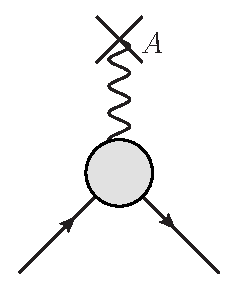
\includegraphics[scale=0.4]{../eps/QED-static-field-blob}
    \end{columns}

\begin{itemize}

	\item 	The current $j_\mu = e\bar{\Psi}\Gamma_\mu \Psi$ must
	\begin{itemize}
		\item	transform like a Lorentz 4-vector
		\item	be gauge invariant
	\end{itemize}
	\item	The most general such expression has
\scriptsize\[	\Gamma_\mu = F_e \frac{(p + p' )_\mu}{2m}  - F_m \frac{ \Sigma_{\mu\nu} q^\nu}{2m}	\]\normalsize
	\begin{itemize}
		\item $\Sigma_{\mu \nu}$ is analogous to $\sigma_{\mu\nu}$ in the spin one-half case
		%\item 
		%$\Sigma_{0i} =  \begin{pmatrix} 0 & - \Sigma_i // \Sigma_i & 0 end{pmatrix}$
		%$\Sigma_{ij} = -2i\epsilon_{ijk} \begin{pmatrix} \Sigma_k & 0 \\ 0 & \Sigma_k $
		%TODO fix expressions
		\item The parameters have some dependence on $q$, but at leading order they are $F_e = 1$ and $F_m = g/2$
		\item Other terms can be written, but will not contribute to the NRQED coefficients 
	\end{itemize}
\end{itemize}




\end{frame}
\begin{frame}{Nonrelativistic expansion} %TODO name
To connect back to the NRQED Lagrangian, expand the relativistic expression
\begin{itemize}

\item The wave functions are approximated

\scriptsize
\[
	\Psi \approx \begin{pmatrix}
		\left[1 +  \frac{ (\v{\Sigma} \cdot \v{p})^2}{8m^2} - \frac{\v{p}^2}{4m^2} \right]	\phi	\\
		\frac{\v{\Sigma} \cdot \v{p}}{2m} \phi
	\end{pmatrix}
\] 
\normalsize
\item Example: expand the zero component of the current as
\scriptsize
\[
	\bar{\Psi} \Gamma_0 \Psi \approx
			\phi^\dagger \left( 1 - [g-1]\frac{ (\v{\Sigma} \cdot \v{q})^2}{8m^2} + [g-1]\frac{ i \v{s} \cdot (\v{q} \times \v{p}) }{4m^2} \right ) \phi
\]
\normalsize
\item This then gives rise to terms in the potential
\scriptsize
\[
eA_0 \bar{\Psi} \Gamma_0 \Psi \to
eA_0 - e [g-1] \left(  \frac{\v{\grad} \cdot \v{E}}{8m^2} \frac{\v{\Sigma}^2}{3}  + \lambda \frac{Q_{ij} \grad_i E_j}{4m^2} \right ) - e[g-1] \frac{ \v{s} \cdot \v{E} \times \v{p} }{2m^2}
\]
\normalsize
\end{itemize}
\end{frame}


% \begin{frame}
% \frametitle{NRQED Lagrangian}
% 
% The NRQED Lagrangian has the same general form as for spin one:
% \scriptsize
% 
% \beqa
% 	\mathcal{L} &=& \phi^\dagger \{ i(\partial_0 + ieA_0) + \frac{\v{D}^2}{2m} + \frac{\v{D}^4}{8m^3} 
% 		+ c_F \frac{\v{S} \cdot \v{B}} {2m}   	
% 		+ c_D \frac{ e(\v{D} \cdot \v{E} - \v{E} \cdot \v{D} ) }{8m^2}	\\
% 	&&	+ c_Q \frac{e Q_{ij} (D_i E_j - E_i D_j) }{8m^2}	
% 		+ c_S \frac{ ie \v{S} \cdot ( \v{D} \times \v{E} - \v{E} \times \v{D} )}{8m^2}
% 		+ c_{W_1} \frac{ e [ \v{D}^2 (\v{S} \cdot \v{B} ) + (\v{S} \cdot \v{B} ) \v{D}^2] }{8m^3}	\\
% 	&&	- c_{W_2} \frac{ e D^i (\v{S} \cdot \v{B} ) D^i }{4m^3}
% 		+ c_{p'p} \frac{ e [ (\v{S} \cdot \v{D}) (\v{B} \cdot \v{D}) + (\v{B} \cdot \v{D})(\v{S} \cdot \v{D}) }{8m^3} \} \phi
% \eeqa
% 
% \normalsize
% \end{frame}


\begin{frame}
\frametitle{NRQED coefficients}



\begin{itemize}
  \item Scattering amplitudes compared like before
\end{itemize}

\begin{block}{Coefficients for arbitrary spin}
\begin{columns}[l]
\column{.5 in}
\beqa
	c_F &=& g \\
	c_D &=&	(g-1) \frac{\v{\Sigma}^2}{3} 	\\
	c_Q &=&	-2 \lambda (g-1)	
\eeqa
\column{1 in}
\beqa
	c_S &=& 2(g-1)	\\
	c_{W_1}- c_{W_2} &=& 2	\\
	c_{p'p}	&=&  g-2	
\eeqa
\end{columns}
\end{block}
\Sitem{Coefficients before spin trilinears $c_T$ do not appear}

\normalsize
\begin{itemize}
 
 \item $\v{\Sigma^2}$ and $\lambda$ are spin dependent constants
 \item Coefficients for spins 1/2 and 1 agree with previous results
 \item Spin dependence associated with derivatives of the electric field
\end{itemize}



\end{frame}


\begin{frame}
\frametitle{Connection to BMT equation}
\begin{itemize}
	\item 	Universality of some coefficients can be understood through the BMT equation
	\item 	Gives time evolution of spin four-vector $a_\mu$
	\item 	Neglecting derivatives of the electromagnetic field, the equation has no dependence on spin magnitude:
	\beq
		\d{a^\mu}{\tau} = 
		g \frac{e }{2m} F^{\mu\nu} a_\nu - (g-2) \frac{e }{2m} u^\nu F^{\mu \lambda} u_\mu a_\lambda.
	\eeq 
	\item Time evolution of spin must also be given by $[H, \v{S}]$
	\item So to agree with the BMT equation, all relevant coefficients in $H$ must be universal
\end{itemize}
\end{frame}



\begin{frame}
\frametitle{Interaction}
Now we're ready to consider the bound system
\pause
\begin{itemize}
  \item Idea is to calculate $g_b$ with a regular quantum mechanical Hamiltonian \pause
  \item The potential between the two bound particles is found by considering scattering \pause
  \item That scattering is calculated from the NRQED Lagrangian already developed
\end{itemize}

\end{frame}



\begin{frame}
\frametitle{Interaction}
In the absence of an external field, the effective interaction potential can be found from the scattering amplitudes
\begin{columns}
\column{1in}
\begin{center} 
 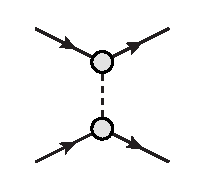
\includegraphics[scale=0.6]{../eps/DashBreit}
 
 
\footnotesize Coulomb exchange \normalsize
 \end{center}

\column{1.5in}
\begin{center}  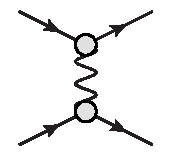
\includegraphics[scale=0.6]{../eps/WaveBreit}
 
\footnotesize Transverse exchange
 \normalsize
 \end{center}
\end{columns}

\vspace{1em}

\footnotesize
\hspace{2em}\mbox{
\begin{minipage}{.7in}
   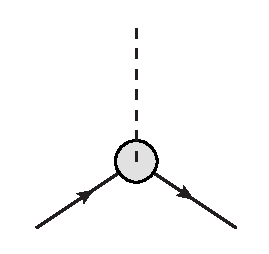
\includegraphics[scale=0.3]{../eps/DashVertexNRQED} 
\end{minipage}
 = \hspace{.5em} $ i e \Big ( 1 + \frac{1}{8m^2} \big [  c_D \v{q}^2 + c_Q Q_{ij} q_i q_j - 2 i c_S \v{S} \cdot \v{p} \times \v{q} \big ]\Big)$
}


\hspace{2em}\mbox{
\begin{minipage}{.7in}
   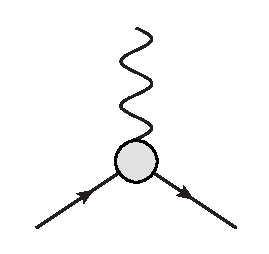
\includegraphics[scale=0.3]{../eps/WaveVertexNRQED} 
\end{minipage}
 = \hspace{1em} $ i\frac{e}{2m} \Big ( \v{p} + \v{p'} + c_F i \v{S} \times \v{q} \Big)_i$.
}

\normalsize







\end{frame}



\begin{frame}
\frametitle{Potential in absence of external field}

\begin{itemize}
\item The scattering is related to the quantum mechanical potential via $M = (\phi^\dagger_1 \phi^\dagger_2 \phi_2 \phi_1) U(\v{p_1}, \v{p_2}, \v{q})$

\item The potential calculated in this way is
\end{itemize}
\footnotesize
\beqa
	\overline{U}(\v{p_1}, \v{p_2}, \v{r}) &=& 	
	 e_1 e_2 \Bigg[ 
		\frac{1}{4\pi r} 
		- \frac{1}{8m_2^2}\left ( d_D \delta(\v{r})  - 3 d_Q \frac{{Q_2}_{ij} r_i r_j}{4 \pi r^5}   - d_S \frac{\v{r} \cdot \v{S_2} \times \v{p_2} }{2\pi r^3}   \right )
 	\\&&	- \frac{1}{8m_1^2}\left ( c_D \delta(\v{r}) - 3 c_Q \frac{{Q_1}_{ij} r_i r_j}{4 \pi r^5}  + c_S \frac{\v{r} \cdot \v{S_1} \times \v{p_1} }{2\pi r^3}   \right )
	\\&&	- \frac{1}{m_1 m_2}\left( \frac{\v{p_1} \cdot \v{p_2}}{8\pi r} + \frac{(\v{p_1} \cdot \v{r}) (\v{p_2} \cdot \v{r}) }{8 \pi r^3}  \right ) 
	\\&&	+ \frac{1}{2 m_1 m_2} \frac{ \v{r} \cdot ( d_F \v{S_2} \times \v{p_1} - c_F \v{S_1} \times \v{p_2} )}{4\pi r^3}
	\\&&	- \frac{c_F d_F }{4 m_1 m_2}\bigg( \frac{2}{3} \v{S_1} \cdot \v{S_2} \delta(\v{r}) 
			- \frac{1}{4\pi r^3} \left\{ \v{S_1} \cdot \v{S_2} - 3 \frac{(\v{S_1} \cdot \v{r}) (\v{S_2} \cdot \v{r}) }{r^2}  \right \}  \bigg)
	\Bigg].
\eeqa
\normalsize

\end{frame}


\begin{frame}
\frametitle{Diagrams with magnetic field}
Now also include the magnetic field, with diagrams like:
\begin{columns}
\column{1in}
\begin{center}  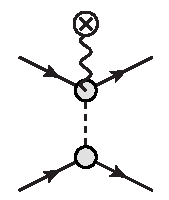
\includegraphics[scale=0.7]{../eps/DashBreitA1} \end{center}
\column{1in}
\begin{center}  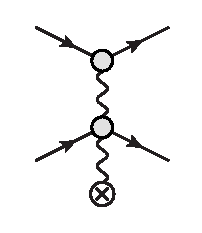
\includegraphics[scale=0.7]{../eps/WaveBreitA2} \end{center}
\end{columns}

\vspace{1em}

Where the new vertices are
\vspace{1em}

\hspace{2em}\mbox{
	\begin{minipage}{1in}
	   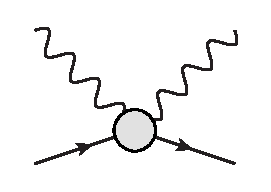
\includegraphics[scale=0.4]{../eps/WaveWaveVertex} 
	\end{minipage}
	$ =  -i\frac{e^2 \delta_{ij}}{m} $.
}

\hspace{2em}\mbox{
	\begin{minipage}{1in}
	   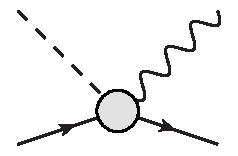
\includegraphics[scale=0.4]{../eps/DashWaveVertex} 
	\end{minipage}
	$ =  c_S \frac{e^2}{4m^2} \epsilon_{ijk} {q_j S_k} $.
}




\end{frame}



\begin{frame}
\frametitle{Interaction potential with magnetic field}

Result in momentum space:
\footnotesize
\beqa
U_2(\v{p_1}, \v{p_2}, \v{q}) &=& 	 e_1 e_2   \Big\{
	- i c_s \frac{e_1}{4m_1^2} \frac{\v{S_1} \cdot \v{A}_1 \times \v{q} }{\v{q}^2}
	+ i d_S \frac{e_2}{4m_2^2} \frac{\v{S_2} \cdot \v{A}_2 \times \v{q} }{\v{q}^2}
\\&&	+\frac{e_1}{ m_1 m_2} \Big ( 
		\frac{ \v{p}_2  \cdot \v{A}_1 }{\v{q}^2} 
		- i d_F \frac{ \v{S}_2 \cdot \v{q} \times \v{A}_1 }{2\v{q}^2} 
		- \frac{ (\v{p}_2 \cdot \v{q}) (\v{A}_1 \cdot \v{q}) }{\v{q}^4 }
	\Big )
\\&&	+\frac{e_2}{ m_1 m_2} \Big ( 
			\frac{ \v{p}_1  \cdot \v{A}_2 }{\v{q}^2} 
			+ i c_F \frac{ \v{S}_1 \cdot \v{q} \times \v{A}_2 }{2\v{q}^2} 
			- \frac{ (\v{p}_1 \cdot \v{q}) (\v{A}_2 \cdot \v{q}) }{\v{q}^4 }
	\Big)
\Big\}
\eeqa 
\normalsize

\end{frame}

\begin{frame}
\frametitle{Relevant part of Hamiltonian}
Full Hamiltonian is  $H = H_1 + H_2 + H_\text{int}$ --- each particle's free Hamiltonian added to the interaction 
\begin{itemize}
  \item Extract relevant parts for particle $1$
  \item Only terms linear in the magnetic field and spin ($S_1$) contribute to $g_b$
  \item \emph{Note}: no spin dependent coefficients enter this expression
\end{itemize}
  
\footnotesize
\beq
\begin{split}
	H^{(1)}_\text{spin} =&
		-g_1 \frac{e_1}{2m_1} \v{S}_1 \cdot \v{B} \left( 1 - \frac{ \v{p}_1^2 }{2m_1^2} \right )
		\\&-(g_1-2) \frac{e_1}{2m^2_1} \v{S}_1 \cdot \v{B} \frac{\v{p}_1^2 }{2m_1^2} 
		+ (g_1-2)  \frac{e_1}{2m^2_1} \frac{( \v{p}_1 \cdot \v{B})(\v{S}_1 \cdot \v{p}_1 )}{2m_1^2}
		\\& -e_1 e_2 (g_1 -1) \frac{ 2 \v{S}_1 \cdot \v{r} \times [\v{p}_1 -e_1\v{A}_1 ] }{16 \pi m_1^2 r^3}
		-e_1 e_2 g_1 \frac{ 2 \v{S}_1 \cdot \v{r} \times [\v{p}_2 -e_2\v{A}_2 ] }{16 \pi m_1 m_2 r^3}.
\end{split}
\eeq
\normalsize

\end{frame}



\begin{frame}
\frametitle{Separation of CoM motion in presence of an external field}
\begin{itemize}
  \item 	Need to separate center of mass motion from internal motion
  \item 	Normal procedure is to define internal/CoM position and momentum as
  	\beq
		\v{r} = \v{r}_1 - \v{r}_2 , \hspace{4em}   \v{R} = \mu_1 \v{r}_1 + \mu_2 \v{r}_2,
	\eeq
	\beq
		\v{p} = \mu_2 \v{p}_1 - \mu_1 \v{p}_2, \hspace{4em}   \v{P} = \v{p}_1 + \v{p}_2
	\eeq
  \item  	External field $\v{A}(\v{r}) = \v{B} \times \v{r} /2$ spoils this separation
  \item 	Solution: additional transformation needed 
\end{itemize}
\end{frame}

\begin{frame}
\frametitle{Transformation}
	Find transformation by demanding the center of mass motion match that of a single particle
	\begin{columns}[t]
	\column{2in} 
		\begin{block}{No field}\begin{center}
		\beq H = \frac{\v{p}^2}{2m}\eeq
		\v{p} is conserved
		\end{center} \end{block}
	
	\column{2in} 
	\begin{block}{With field}	\begin{center}	
		\beq H = \frac{ (\v{p}-e\v{A})^2}{2m} \eeq
		$\v{p} + \v{A}$ is conserved \end{center}
		\end{block}
	\end{columns}
	\small
	\begin{itemize}
		\item In this case of constant magnetic field, can define $\v{A}_R = \mu_1 \v{A}_1 + \mu_2 \v{A}_2$, potential at $\v{R}$.
		\item If the center of mass motion is separated, $\v{P} + e\v{A}_R$ should be conserved
		\item Instead $\v{P} + e(\v{A}_1 + \v{A}_2)$ is the conserved quantity
	\end{itemize}
	\normalsize
\end{frame}

\begin{frame}
\frametitle{Transformation}

Desired quantity is conserved if 
\beq
	\v{P} \to U^{-1} \v{P} U = \v{P} - (e_1 \mu_2 - e_2 \mu_1)\v{A}_r
\eeq
Transformation realised by
\beq
	U = e^{-i(e_1\mu_2 - e_2 \mu_1) \v{A}_R \cdot \v{r}}.
\eeq
Other effects of $U$:
\beqa
	\v{p}_1 &\to& \v{p}_1 + (e_1 \mu_2 - e_2 \mu_1) \v{A}_1		\\
	\v{p}_2 &\to&  \v{p}_2 - (e_1 \mu_2 - e_2 \mu_1) \v{A}_2	\\			
	\v{p} &\to& \v{p} + (e_1 \mu_2 - e_2 \mu_1) \v{A}_R
\eeqa

\end{frame}




\begin{frame}
\frametitle{Transformed Hamiltonian}

\footnotesize

To transform the original Hamiltonian, including perturbations, apply these substitutions.

\beqa
	\v{p}_1 - e_1 \v{A}(\v{r}_1) &\to&	 \mu_1 [ \v{P} - (e_1 + e_2)\v{A}(\v{R}) ] +  \left[\v{p} - [e_1 -(e_1+e_2)\mu_1^2  ] \v{A}(\v{r}) \right ],	\\
	\v{p}_2 -e_2 \v{A}(\v{r}_1) &\to&	\mu_2	 [ \v{P} - (e_1 + e_2)\v{A}(\v{R}) ] +  \left[\v{p} - [e_2 -(e_1+e_2)\mu_2^2  ] \v{A}(\v{r}) \right ]	
\eeqa
\begin{block}{Resultant Hamiltonian}

\beq \label{eq:Br:H}
\begin{split}
 H'^{(1)}_\text{spin} =&
 -g_1 \frac{e_1}{2m_1} \v{S}_1 \cdot \v{B} \left( 1 - \frac{ \v{p}^2 }{2m_1^2} \right )
		\\& -(g_1-2) \frac{e_1}{2m^2_1} \v{S}_1 \cdot \v{B} \frac{\v{p}^2 }{2m_1^2} 
		 + (g_1-2)  \frac{e_1}{2m^2_1} \frac{( \v{p} \cdot \v{B})(\v{S}_1 \cdot \v{p} )}{2m_1^2}
		\\& -e_1 e_2 (g_1 -1) \frac{ 2 \v{S}_1 \cdot \v{r} \times [\v{p} - (e_1-[e_1 + e_2]\mu_1^2 )\v{A}_r ] }{16 \pi m_1^2 r^3}
		\\& -e_1 e_2 g_1 \frac{ 2 \v{S}_1 \cdot \v{r} \times [\v{p} -(e_2-[e_1 + e_2]\mu_2^2 ) \v{A}_r ] }{16 \pi m_1 m_2 r^3}.
\end{split}
\eeq
\normalsize
\end{block}


\end{frame}

\begin{frame}
\frametitle{Calculation of $g_b$}
\begin{itemize}
  \item	Calculate $g_b$ for $S$-states of hydrogen like systems
  \item Calculate matrix elements like
  	\footnotesize
%   	\beq
% 		\v{S} \cdot \v{r} \times \v{A} \to \frac{1}{3}  \v{S} \cdot \v{B} r^2
% 	\eeq
  	\beq
		\matrixel{n}{\frac{1}{r}}{n} = - \frac{m_r e_1 e_2 }{4\pi n^2} = \frac{m_r Z\alpha}{n^2}, \hspace{2em}
		\matrixel{n}{\v{p}^2}{n} = \frac{ m_r^2  e_1^2 e_2^2}{16 \pi^2 n^2} = \frac{m_r^2  (Z\alpha)^2}{n^2}.
	\eeq
	
	\normalsize
	\item  $g_2^\text{bound}$ found by exchange of indices 
  \end{itemize}
  \footnotesize

  \begin{block}{Bound $g$ with recoil and binding corrections}
  \beq 
\begin{split}
g_1^\text{bound} =& g_1 \Bigg \{
			\left( 1 - \frac{ \mu_2^2 (Z\alpha)^2}{2n^2} \right )
			+ \frac{ 	\mu_2^2 Z^2 \alpha [ \alpha + (Z\alpha - \alpha)\mu_1^2 ] }{6n^2}
		\\&	- \frac{ \mu_1^2 Z^2 \alpha [Z\alpha + (Z\alpha - \alpha)\mu_2^2 ]}{3n^2} \Bigg \}
		\\& + (g_1 - 2) \Bigg \{
			\frac{ \mu_2^2 (Z\alpha)^2 }{3n^2}
			+ \frac{ \mu_2^2 Z^2 \alpha[ \alpha + ( Z\alpha - \alpha) \mu_1^2)\mu_1^2 ] }{6n^2} \Bigg \}
\end{split}
\eeq  \normalsize \end{block}

\end{frame}



\begin{frame}
\frametitle{Results}
\begin{itemize}
  \item  NRQED Lagrangian for arbitrary spin up to $\mathcal{O}(1/m^3)$ was developed
  \item  Agrees with known NRQED Lagrangians for spin one and spin one-half
  \item  Quantum mechanical Hamiltonian obtained for two particles of arbitrary spin in a loosely bound system
  \item  Leading order binding and recoil corrections for $g_b$ calculated
  \item  Such corrections were shown to be universal (no dependence on spin magnitude)
  \item  Physical reason for universality related to BMT equation
\end{itemize}
\end{frame}


\end{document}
